\documentclass[12pt]{article}
\usepackage{placeins}
\usepackage{sbc-template}
\usepackage{float}
\usepackage{graphicx,url}
\usepackage{listings}
\usepackage{longtable}
\usepackage{lscape}
\usepackage{multirow}
\usepackage[brazil]{babel}   
%\usepackage[latin1]{inputenc}  
\usepackage[utf8]{inputenc} 
\usepackage{color}
\usepackage{geometry}
\definecolor{dkgreen}{rgb}{0,0.6,0}
\definecolor{gray}{rgb}{0.5,0.5,0.5}
\definecolor{mauve}{rgb}{0.58,0,0.82}
 
% UTF-8 encoding is recommended by ShareLaTex

\sloppy
\lstset{
  language=Python,                
  basicstyle=\footnotesize,           
  numbers=left,                   
  numberstyle=\tiny\color{gray},  
  stepnumber=2,                             
  numbersep=5pt,                  
  backgroundcolor=\color{white},    
  showspaces=false,               
  showstringspaces=false,         
  showtabs=false,                 
  frame=single,                   
  rulecolor=\color{black},        
  tabsize=2,                      
  captionpos=b,                   
  breaklines=true,                
  breakatwhitespace=false,        
  title=\lstname,                               
  keywordstyle=\color{blue},          
  commentstyle=\color{dkgreen},       
  stringstyle=\color{mauve}, }


\title{Projeto de Comunicações Móveis}

\author{Vítor Gabriel Lemos Lopes}


\address{Departamento de Engenharia de Comunicações-UFRN
}

\begin{document} 

\maketitle

     
\begin{resumo} 
  Este Trabalho foi feito com intuito de aprendizado adaptação de enlace e conhecimento sobre Long Term Evolution(LTE), Mapeando as possíveis taxas de transmissão dada uma SINR . Para isso foi utilizado a linguagem de programação em Python para a modelagem dos possíveis valores de SINR, com isso foram feitos gráficos para comparação entre o Release 8 e 10 do 3GPP.
\end{resumo}
\section{Introdução}
Nos sistemas do 3GPP, cada um tem sua forma de calcular taxa de transmissão, aqui abordaremos sobre o LTE(\textit{Long Term Evolution}), ou também conhecido como 4G. Para poder calcularmos a taxa de transmissão, precisamos saber quem é MCS(\textit{Modulation and Coding Scheme}) que é quem quem vai mapear a modulação e a taxa de codificação, e o MCS é mapeado de acordo com a CQI(\textit{Channel Quality Indicator}), que para cada faixa de SNR temos um CQI diferente, e a SNR é dada por cada usuário, e para ficar com uma melhor \textit{throughput},para isso usamos essa tabela:\cite{CQISNR}
\begin{figure}[h]
    \centering
    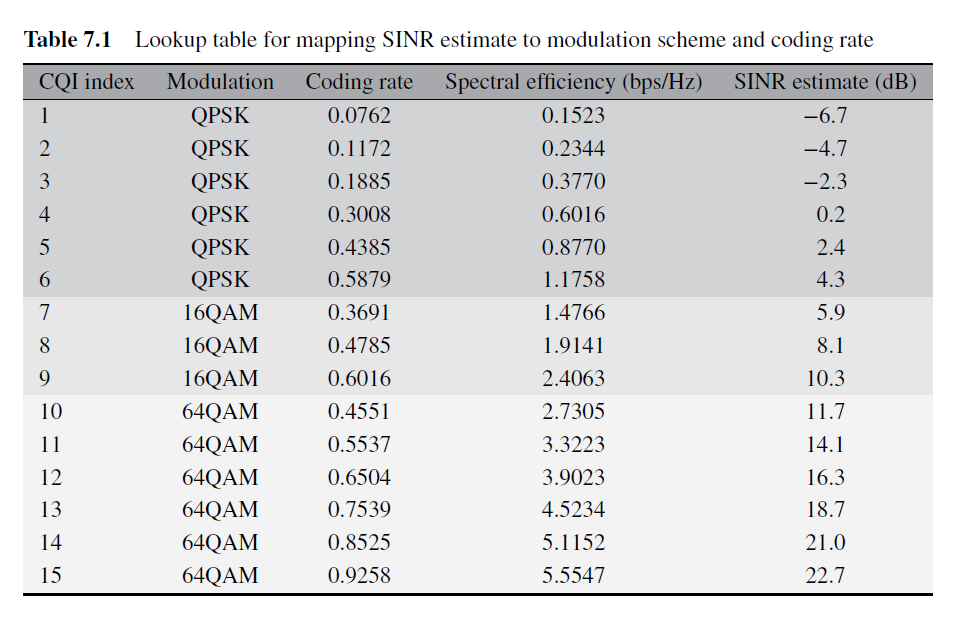
\includegraphics[width=0.75\textwidth]{SINRestimateLTEBook.png}
    \caption{Mapeando CQI dada SNR}
    \label{fig:my_label}
\end{figure}
\FloatBarrier
De posse da tabela acima temos só que fazer um mapeamento de CQI em MCS, o qual utilizamos o da patente: \cite{Patente}
\begin{figure}[h]
    \centering
    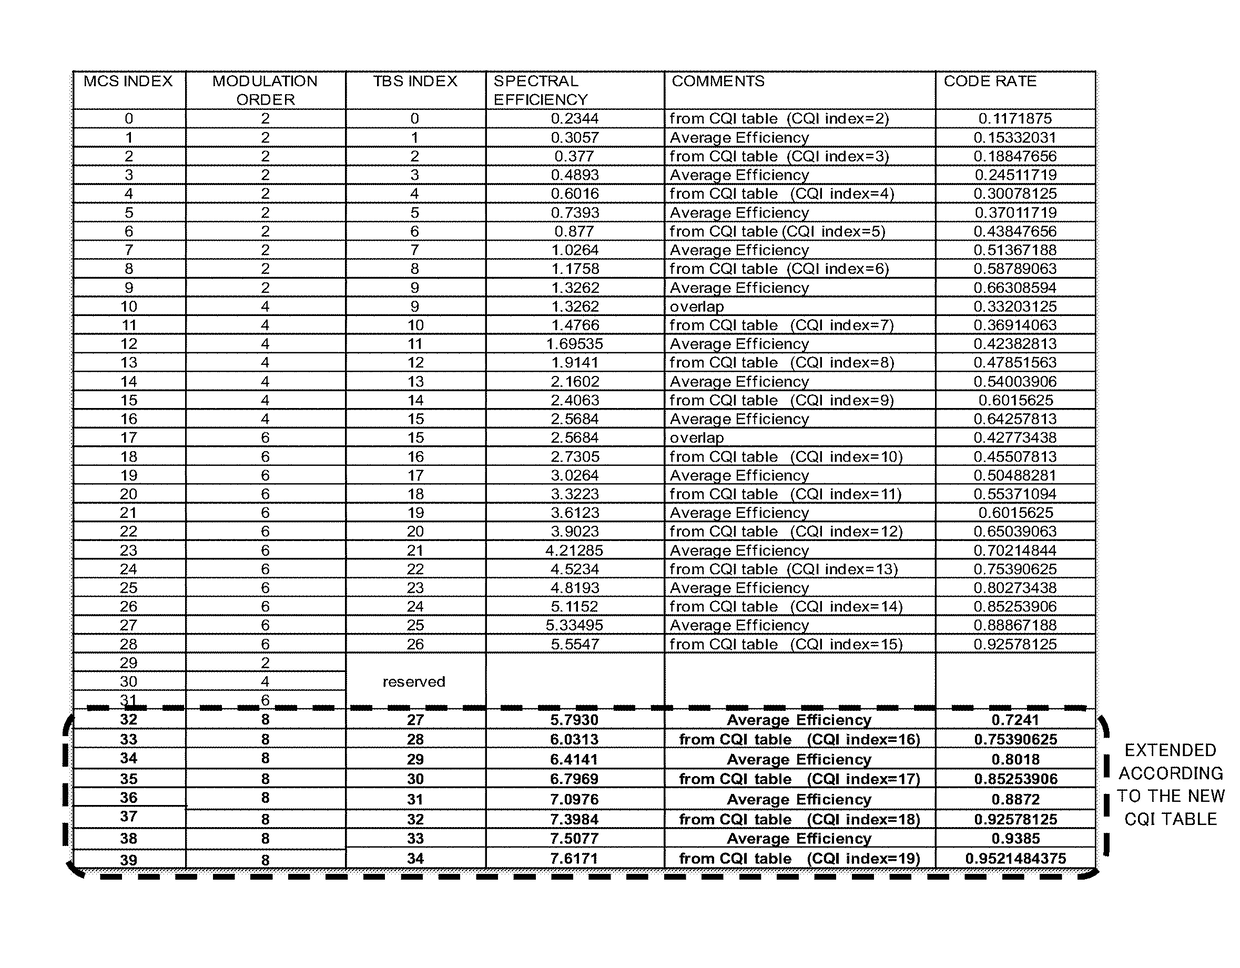
\includegraphics[width=1.2\textwidth]{US10136451-D00000.png}
    \caption{Mapeando MCS em CQI}
    \label{fig:my_label}
\end{figure}
\FloatBarrier
\section{Experimento 1} \label{sec:firstpage}
No primeiro experimento foi pedido para que fosse apresentado as tabelas de taxa de pico através da formula e da tabela, com o mapeamento feito na introdução, conseguimos montar a formula da taxa de transmissão. Sabendo que a banda de 1.4Mhz são 6 PRBs, 3Mhz são 15 PRBs, 5Mhz são 25 PRBs,10Mhz são 50 PRBs e 20MHZ são 100 PRBs\cite{calctab}. A formula é:
\begin{equation}
    Tput=mimo*prb*cp*12*mod*0.75*ca*cod/(0.5*10^{-3})
\end{equation}
O quais:
\begin{itemize}
    \item mimo=Número de antenas
    \item prb=Número de prbs
    \item cp=se é prefixo normal(7) se for estendido(6)
    \item 12 é o numero de subportadoras
    \item mod= a modulação usada em $log_{2}(Qam)$
    \item 0.75 é porque 0.25 é a overhead \cite{Overhead25}
    \item ca= é o número dos carrier aggregation, que release 8 é 1.
    \item cod= a taxa de codificação 
    \item 0.5*10$^{-3}$ é o tempo do slot
\end{itemize}
Com posse do calculo pela formula,só precisamos definir como se calcula pela tabela da norma do 3GPP\cite{ts36213} que é dado por esse site \cite{calctab},que é o valor dos bits do TBS index e o MCS, multiplicado por 1000. Com posse desses dados podemos montar essa tabela para o release 8.
\fontsize{5}{6}\selectfont 
% Please add the following required packages to your document preamble:
% \usepackage{multirow}
% \usepackage{longtable}
% Note: It may be necessary to compile the document several times to get a multi-page table to line up properly
\begin{longtable}[c]{|l|l|l|l|l|l|l|l|l|l|l|l|l|l|}
\hline
\multirow{3}{*}{MCS} & \multirow{3}{*}{MIMO} &35
 \multicolumn{12}{l|}{Taxa de transmissão} \\ \cline{3-14} 
 &  & 1.4MHZ & 1.4MHZ & 3MHZ & 3MHZ & 5MHZ & 5MHZ & 10MHZ & 10MHZ & 15MHZ & 15MHZ & 20MHZ & 20MHZ \\ \cline{3-14} 
 &  & Equação & Tabela & Equação & Tabela & Equação & Tabela & Equação & Tabela & Equação & Tabela & Equação & Tabela \\ \hline
\endfirsthead
%
\multicolumn{14}{c}%
{{\bfseries Table \thetable\ continued from previous page}} \\
\endhead
%
0 & 1x1 & 177.19 kbps & 152.00 kbps & 442.97 kbps & 392.00 kbps & 738.28 kbps & 680.00 kbps & 1.48 Mbps & 1.38 Mbps & 2.21 Mbps & 2.09 Mbps & 2.95 Mbps & 2.79 Mbps \\ \hline
0 & 2x2 & 354.38 kbps & 304.00 kbps & 885.94 kbps & 784.00 kbps & 1.48 Mbps & 1.36 Mbps & 2.95 Mbps & 2.77 Mbps & 4.43 Mbps & 4.18 Mbps & 5.91 Mbps & 5.58 Mbps \\ \hline
0 & 4x4 & 708.75 kbps & 608.00 kbps & 1.77 Mbps & 1.57 Mbps & 2.95 Mbps & 2.72 Mbps & 5.91 Mbps & 5.54 Mbps & 8.86 Mbps & 8.35 Mbps & 11.81 Mbps & 11.17 Mbps \\ \hline
1 & 1x1 & 231.82 kbps & 208.00 kbps & 579.55 kbps & 520.00 kbps & 965.92 kbps & 904.00 kbps & 1.93 Mbps & 1.80 Mbps & 2.90 Mbps & 2.73 Mbps & 3.86 Mbps & 3.62 Mbps \\ \hline
1 & 2x2 & 463.64 kbps & 416.00 kbps & 1.16 Mbps & 1.04 Mbps & 1.93 Mbps & 1.81 Mbps & 3.86 Mbps & 3.60 Mbps & 5.80 Mbps & 5.46 Mbps & 7.73 Mbps & 7.25 Mbps \\ \hline
1 & 4x4 & 927.28 kbps & 832.00 kbps & 2.32 Mbps & 2.08 Mbps & 3.86 Mbps & 3.62 Mbps & 7.73 Mbps & 7.20 Mbps & 11.59 Mbps & 10.91 Mbps & 15.45 Mbps & 14.50 Mbps \\ \hline
2 & 1x1 & 284.98 kbps & 256.00 kbps & 712.44 kbps & 648.00 kbps & 1.19 Mbps & 1.10 Mbps & 2.37 Mbps & 2.22 Mbps & 3.56 Mbps & 3.37 Mbps & 4.75 Mbps & 4.58 Mbps \\ \hline
2 & 2x2 & 569.95 kbps & 512.00 kbps & 1.42 Mbps & 1.30 Mbps & 2.37 Mbps & 2.19 Mbps & 4.75 Mbps & 4.43 Mbps & 7.12 Mbps & 6.74 Mbps & 9.50 Mbps & 9.17 Mbps \\ \hline
2 & 4x4 & 1.14 Mbps & 1.02 Mbps & 2.85 Mbps & 2.59 Mbps & 4.75 Mbps & 4.38 Mbps & 9.50 Mbps & 8.86 Mbps & 14.25 Mbps & 13.47 Mbps & 19.00 Mbps & 18.34 Mbps \\ \hline
3 & 1x1 & 370.62 kbps & 328.00 kbps & 926.54 kbps & 872.00 kbps & 1.54 Mbps & 1.42 Mbps & 3.09 Mbps & 2.86 Mbps & 4.63 Mbps & 4.39 Mbps & 6.18 Mbps & 5.74 Mbps \\ \hline
3 & 2x2 & 741.23 kbps & 656.00 kbps & 1.85 Mbps & 1.74 Mbps & 3.09 Mbps & 2.83 Mbps & 6.18 Mbps & 5.71 Mbps & 9.27 Mbps & 8.78 Mbps & 12.35 Mbps & 11.47 Mbps \\ \hline
3 & 4x4 & 1.48 Mbps & 1.31 Mbps & 3.71 Mbps & 3.49 Mbps & 6.18 Mbps & 5.66 Mbps & 12.35 Mbps & 11.42 Mbps & 18.53 Mbps & 17.57 Mbps & 24.71 Mbps & 22.94 Mbps \\ \hline
4 & 1x1 & 454.68 kbps & 408.00 kbps & 1.14 Mbps & 1.06 Mbps & 1.89 Mbps & 1.80 Mbps & 3.79 Mbps & 3.62 Mbps & 5.68 Mbps & 5.35 Mbps & 7.58 Mbps & 7.22 Mbps \\ \hline
4 & 2x2 & 909.35 kbps & 816.00 kbps & 2.27 Mbps & 2.13 Mbps & 3.79 Mbps & 3.60 Mbps & 7.58 Mbps & 7.25 Mbps & 11.37 Mbps & 10.70 Mbps & 15.16 Mbps & 14.45 Mbps \\ \hline
4 & 4x4 & 1.82 Mbps & 1.63 Mbps & 4.55 Mbps & 4.26 Mbps & 7.58 Mbps & 7.20 Mbps & 15.16 Mbps & 14.50 Mbps & 22.73 Mbps & 21.41 Mbps & 30.31 Mbps & 28.90 Mbps \\ \hline
5 & 1x1 & 559.62 kbps & 504.00 kbps & 1.40 Mbps & 1.32 Mbps & 2.33 Mbps & 2.22 Mbps & 4.66 Mbps & 4.39 Mbps & 7.00 Mbps & 6.71 Mbps & 9.33 Mbps & 8.76 Mbps \\ \hline
5 & 2x2 & 1.12 Mbps & 1.01 Mbps & 2.80 Mbps & 2.64 Mbps & 4.66 Mbps & 4.43 Mbps & 9.33 Mbps & 8.78 Mbps & 13.99 Mbps & 13.42 Mbps & 18.65 Mbps & 17.52 Mbps \\ \hline
5 & 4x4 & 2.24 Mbps & 2.02 Mbps & 5.60 Mbps & 5.28 Mbps & 9.33 Mbps & 8.86 Mbps & 18.65 Mbps & 17.57 Mbps & 27.98 Mbps & 26.85 Mbps & 37.31 Mbps & 35.04 Mbps \\ \hline
6 & 1x1 & 662.98 kbps & 600.00 kbps & 1.66 Mbps & 1.54 Mbps & 2.76 Mbps & 2.60 Mbps & 5.52 Mbps & 5.16 Mbps & 8.29 Mbps & 7.74 Mbps & 11.05 Mbps & 10.30 Mbps \\ \hline
6 & 2x2 & 1.33 Mbps & 1.20 Mbps & 3.31 Mbps & 3.09 Mbps & 5.52 Mbps & 5.20 Mbps & 11.05 Mbps & 10.32 Mbps & 16.57 Mbps & 15.47 Mbps & 22.10 Mbps & 20.59 Mbps \\ \hline
6 & 4x4 & 2.65 Mbps & 2.40 Mbps & 6.63 Mbps & 6.18 Mbps & 11.05 Mbps & 10.40 Mbps & 22.10 Mbps & 20.64 Mbps & 33.15 Mbps & 30.94 Mbps & 44.20 Mbps & 41.18 Mbps \\ \hline
7 & 1x1 & 776.67 kbps & 712.00 kbps & 1.94 Mbps & 1.80 Mbps & 3.24 Mbps & 3.11 Mbps & 6.47 Mbps & 6.20 Mbps & 9.71 Mbps & 9.14 Mbps & 12.94 Mbps & 12.22 Mbps \\ \hline
7 & 2x2 & 1.55 Mbps & 1.42 Mbps & 3.88 Mbps & 3.60 Mbps & 6.47 Mbps & 6.22 Mbps & 12.94 Mbps & 12.40 Mbps & 19.42 Mbps & 18.29 Mbps & 25.89 Mbps & 24.43 Mbps \\ \hline
7 & 4x4 & 3.11 Mbps & 2.85 Mbps & 7.77 Mbps & 7.20 Mbps & 12.94 Mbps & 12.45 Mbps & 25.89 Mbps & 24.80 Mbps & 38.83 Mbps & 36.58 Mbps & 51.78 Mbps & 48.86 Mbps \\ \hline
8 & 1x1 & 888.89 kbps & 808.00 kbps & 2.22 Mbps & 2.09 Mbps & 3.70 Mbps & 3.50 Mbps & 7.41 Mbps & 6.97 Mbps & 11.11 Mbps & 10.68 Mbps & 14.81 Mbps & 14.11 Mbps \\ \hline
8 & 2x2 & 1.78 Mbps & 1.62 Mbps & 4.44 Mbps & 4.18 Mbps & 7.41 Mbps & 6.99 Mbps & 14.81 Mbps & 13.94 Mbps & 22.22 Mbps & 21.36 Mbps & 29.63 Mbps & 28.22 Mbps \\ \hline
8 & 4x4 & 3.56 Mbps & 3.23 Mbps & 8.89 Mbps & 8.35 Mbps & 14.81 Mbps & 13.98 Mbps & 29.63 Mbps & 27.87 Mbps & 44.44 Mbps & 42.72 Mbps & 59.26 Mbps & 56.45 Mbps \\ \hline
9 & 1x1 & 1.00 Mbps & 936.00 kbps & 2.51 Mbps & 2.34 Mbps & 4.18 Mbps & 4.01 Mbps & 8.35 Mbps & 7.99 Mbps & 12.53 Mbps & 11.83 Mbps & 16.71 Mbps & 15.84 Mbps \\ \hline
9 & 2x2 & 2.01 Mbps & 1.87 Mbps & 5.01 Mbps & 4.69 Mbps & 8.35 Mbps & 8.02 Mbps & 16.71 Mbps & 15.98 Mbps & 25.06 Mbps & 23.66 Mbps & 33.42 Mbps & 31.68 Mbps \\ \hline
9 & 4x4 & 4.01 Mbps & 3.74 Mbps & 10.03 Mbps & 9.38 Mbps & 16.71 Mbps & 16.03 Mbps & 33.42 Mbps & 31.97 Mbps & 50.13 Mbps & 47.33 Mbps & 66.84 Mbps & 63.36 Mbps \\ \hline
10 & 1x1 & 1.00 Mbps & 936.00 kbps & 2.51 Mbps & 2.34 Mbps & 4.18 Mbps & 4.01 Mbps & 8.37 Mbps & 7.99 Mbps & 12.55 Mbps & 11.83 Mbps & 16.73 Mbps & 15.84 Mbps \\ \hline
10 & 2x2 & 2.01 Mbps & 1.87 Mbps & 5.02 Mbps & 4.69 Mbps & 8.37 Mbps & 8.02 Mbps & 16.73 Mbps & 15.98 Mbps & 25.10 Mbps & 23.66 Mbps & 33.47 Mbps & 31.68 Mbps \\ \hline
10 & 4x4 & 4.02 Mbps & 3.74 Mbps & 10.04 Mbps & 9.38 Mbps & 16.73 Mbps & 16.03 Mbps & 33.47 Mbps & 31.97 Mbps & 50.20 Mbps & 47.33 Mbps & 66.94 Mbps & 63.36 Mbps \\ \hline
11 & 1x1 & 1.12 Mbps & 1.03 Mbps & 2.79 Mbps & 2.66 Mbps & 4.65 Mbps & 4.39 Mbps & 9.30 Mbps & 8.76 Mbps & 13.95 Mbps & 12.96 Mbps & 18.60 Mbps & 17.57 Mbps \\ \hline
11 & 2x2 & 2.23 Mbps & 2.06 Mbps & 5.58 Mbps & 5.33 Mbps & 9.30 Mbps & 8.78 Mbps & 18.60 Mbps & 17.52 Mbps & 27.91 Mbps & 25.92 Mbps & 37.21 Mbps & 35.14 Mbps \\ \hline
11 & 4x4 & 4.47 Mbps & 4.13 Mbps & 11.16 Mbps & 10.66 Mbps & 18.60 Mbps & 17.57 Mbps & 37.21 Mbps & 35.04 Mbps & 55.81 Mbps & 51.84 Mbps & 74.42 Mbps & 70.27 Mbps \\ \hline
12 & 1x1 & 1.28 Mbps & 1.19 Mbps & 3.20 Mbps & 2.98 Mbps & 5.34 Mbps & 4.97 Mbps & 10.68 Mbps & 9.91 Mbps & 16.02 Mbps & 15.26 Mbps & 21.36 Mbps & 19.85 Mbps \\ \hline
12 & 2x2 & 2.56 Mbps & 2.38 Mbps & 6.41 Mbps & 5.97 Mbps & 10.68 Mbps & 9.94 Mbps & 21.36 Mbps & 19.82 Mbps & 32.04 Mbps & 30.53 Mbps & 42.72 Mbps & 39.70 Mbps \\ \hline
12 & 4x4 & 5.13 Mbps & 4.77 Mbps & 12.82 Mbps & 11.94 Mbps & 21.36 Mbps & 19.87 Mbps & 42.72 Mbps & 39.65 Mbps & 64.08 Mbps & 61.06 Mbps & 85.44 Mbps & 79.39 Mbps \\ \hline
13 & 1x1 & 1.45 Mbps & 1.35 Mbps & 3.62 Mbps & 3.37 Mbps & 6.03 Mbps & 5.74 Mbps & 12.06 Mbps & 11.45 Mbps & 18.09 Mbps & 16.99 Mbps & 24.12 Mbps & 22.92 Mbps \\ \hline
13 & 2x2 & 2.89 Mbps & 2.70 Mbps & 7.24 Mbps & 6.74 Mbps & 12.06 Mbps & 11.47 Mbps & 24.12 Mbps & 22.90 Mbps & 36.18 Mbps & 33.98 Mbps & 48.23 Mbps & 45.84 Mbps \\ \hline
13 & 4x4 & 5.79 Mbps & 5.41 Mbps & 14.47 Mbps & 13.47 Mbps & 24.12 Mbps & 22.94 Mbps & 48.23 Mbps & 45.79 Mbps & 72.35 Mbps & 67.97 Mbps & 96.47 Mbps & 91.68 Mbps \\ \hline
14 & 1x1 & 1.63 Mbps & 1.54 Mbps & 4.08 Mbps & 3.88 Mbps & 6.80 Mbps & 6.46 Mbps & 13.61 Mbps & 12.96 Mbps & 20.41 Mbps & 19.08 Mbps & 27.22 Mbps & 25.46 Mbps \\ \hline
14 & 2x2 & 3.27 Mbps & 3.09 Mbps & 8.17 Mbps & 7.76 Mbps & 13.61 Mbps & 12.91 Mbps & 27.22 Mbps & 25.92 Mbps & 40.83 Mbps & 38.16 Mbps & 54.44 Mbps & 50.91 Mbps \\ \hline
14 & 4x4 & 6.53 Mbps & 6.18 Mbps & 16.33 Mbps & 15.52 Mbps & 27.22 Mbps & 25.82 Mbps & 54.44 Mbps & 51.84 Mbps & 81.65 Mbps & 76.32 Mbps & 108.87 Mbps & 101.82 Mbps \\ \hline
15 & 1x1 & 1.82 Mbps & 1.74 Mbps & 4.55 Mbps & 4.26 Mbps & 7.58 Mbps & 7.22 Mbps & 15.16 Mbps & 14.11 Mbps & 22.74 Mbps & 21.38 Mbps & 30.32 Mbps & 28.34 Mbps \\ \hline
15 & 2x2 & 3.64 Mbps & 3.47 Mbps & 9.10 Mbps & 8.53 Mbps & 15.16 Mbps & 14.45 Mbps & 30.32 Mbps & 28.22 Mbps & 45.48 Mbps & 42.77 Mbps & 60.64 Mbps & 56.67 Mbps \\ \hline
15 & 4x4 & 7.28 Mbps & 6.94 Mbps & 18.19 Mbps & 17.06 Mbps & 30.32 Mbps & 28.90 Mbps & 60.64 Mbps & 56.45 Mbps & 90.96 Mbps & 85.54 Mbps & 121.27 Mbps & 113.34 Mbps \\ \hline
16 & 1x1 & 1.94 Mbps & 1.80 Mbps & 4.86 Mbps & 4.58 Mbps & 8.10 Mbps & 7.74 Mbps & 16.19 Mbps & 15.26 Mbps & 24.29 Mbps & 22.92 Mbps & 32.39 Mbps & 30.58 Mbps \\ \hline
16 & 2x2 & 3.89 Mbps & 3.60 Mbps & 9.72 Mbps & 9.17 Mbps & 16.19 Mbps & 15.47 Mbps & 32.39 Mbps & 30.53 Mbps & 48.58 Mbps & 45.84 Mbps & 64.77 Mbps & 61.15 Mbps \\ \hline
16 & 4x4 & 7.77 Mbps & 7.20 Mbps & 19.43 Mbps & 18.34 Mbps & 32.39 Mbps & 30.94 Mbps & 64.77 Mbps & 61.06 Mbps & 97.16 Mbps & 91.68 Mbps & 129.54 Mbps & 122.30 Mbps \\ \hline
17 & 1x1 & 1.94 Mbps & 1.80 Mbps & 4.85 Mbps & 4.58 Mbps & 8.08 Mbps & 7.74 Mbps & 16.17 Mbps & 15.26 Mbps & 24.25 Mbps & 22.92 Mbps & 32.34 Mbps & 30.58 Mbps \\ \hline
17 & 2x2 & 3.88 Mbps & 3.60 Mbps & 9.70 Mbps & 9.17 Mbps & 16.17 Mbps & 15.47 Mbps & 32.34 Mbps & 30.53 Mbps & 48.51 Mbps & 45.84 Mbps & 64.67 Mbps & 61.15 Mbps \\ \hline
17 & 4x4 & 7.76 Mbps & 7.20 Mbps & 19.40 Mbps & 18.34 Mbps & 32.34 Mbps & 30.94 Mbps & 64.67 Mbps & 61.06 Mbps & 97.01 Mbps & 91.68 Mbps & 129.35 Mbps & 122.30 Mbps \\ \hline
18 & 1x1 & 2.06 Mbps & 1.93 Mbps & 5.16 Mbps & 4.97 Mbps & 8.60 Mbps & 7.99 Mbps & 17.20 Mbps & 16.42 Mbps & 25.80 Mbps & 24.50 Mbps & 34.40 Mbps & 32.86 Mbps \\ \hline
18 & 2x2 & 4.13 Mbps & 3.86 Mbps & 10.32 Mbps & 9.94 Mbps & 17.20 Mbps & 15.98 Mbps & 34.40 Mbps & 32.83 Mbps & 51.61 Mbps & 48.99 Mbps & 68.81 Mbps & 65.71 Mbps \\ \hline
18 & 4x4 & 8.26 Mbps & 7.71 Mbps & 20.64 Mbps & 19.87 Mbps & 34.40 Mbps & 31.97 Mbps & 68.81 Mbps & 65.66 Mbps & 103.21 Mbps & 97.98 Mbps & 137.62 Mbps & 131.42 Mbps \\ \hline
19 & 1x1 & 2.29 Mbps & 2.15 Mbps & 5.73 Mbps & 5.35 Mbps & 9.54 Mbps & 9.14 Mbps & 19.08 Mbps & 18.34 Mbps & 28.63 Mbps & 27.38 Mbps & 38.17 Mbps & 36.70 Mbps \\ \hline
19 & 2x2 & 4.58 Mbps & 4.30 Mbps & 11.45 Mbps & 10.70 Mbps & 19.08 Mbps & 18.29 Mbps & 38.17 Mbps & 36.67 Mbps & 57.25 Mbps & 54.75 Mbps & 76.34 Mbps & 73.39 Mbps \\ \hline
19 & 4x4 & 9.16 Mbps & 8.61 Mbps & 22.90 Mbps & 21.41 Mbps & 38.17 Mbps & 36.58 Mbps & 76.34 Mbps & 73.34 Mbps & 114.51 Mbps & 109.50 Mbps & 152.68 Mbps & 146.78 Mbps \\ \hline
20 & 1x1 & 2.51 Mbps & 2.34 Mbps & 6.28 Mbps & 5.99 Mbps & 10.47 Mbps & 9.91 Mbps & 20.93 Mbps & 19.85 Mbps & 31.40 Mbps & 29.30 Mbps & 41.86 Mbps & 39.23 Mbps \\ \hline
20 & 2x2 & 5.02 Mbps & 4.69 Mbps & 12.56 Mbps & 11.98 Mbps & 20.93 Mbps & 19.82 Mbps & 41.86 Mbps & 39.70 Mbps & 62.79 Mbps & 58.59 Mbps & 83.72 Mbps & 78.46 Mbps \\ \hline
20 & 4x4 & 10.05 Mbps & 9.38 Mbps & 25.12 Mbps & 23.97 Mbps & 41.86 Mbps & 39.65 Mbps & 83.72 Mbps & 79.39 Mbps & 125.58 Mbps & 117.18 Mbps & 167.44 Mbps & 156.93 Mbps \\ \hline
21 & 1x1 & 2.73 Mbps & 2.60 Mbps & 6.82 Mbps & 6.46 Mbps & 11.37 Mbps & 10.68 Mbps & 22.74 Mbps & 21.38 Mbps & 34.11 Mbps & 32.86 Mbps & 45.48 Mbps & 43.82 Mbps \\ \hline
21 & 2x2 & 5.46 Mbps & 5.20 Mbps & 13.64 Mbps & 12.91 Mbps & 22.74 Mbps & 21.36 Mbps & 45.48 Mbps & 42.77 Mbps & 68.22 Mbps & 65.71 Mbps & 90.96 Mbps & 87.63 Mbps \\ \hline
21 & 4x4 & 10.91 Mbps & 10.40 Mbps & 27.29 Mbps & 25.82 Mbps & 45.48 Mbps & 42.72 Mbps & 90.96 Mbps & 85.54 Mbps & 136.43 Mbps & 131.42 Mbps & 181.91 Mbps & 175.26 Mbps \\ \hline
22 & 1x1 & 2.95 Mbps & 2.79 Mbps & 7.38 Mbps & 6.97 Mbps & 12.29 Mbps & 11.45 Mbps & 24.58 Mbps & 22.92 Mbps & 36.88 Mbps & 35.16 Mbps & 49.17 Mbps & 46.89 Mbps \\ \hline
22 & 2x2 & 5.90 Mbps & 5.58 Mbps & 14.75 Mbps & 13.94 Mbps & 24.58 Mbps & 22.90 Mbps & 49.17 Mbps & 45.84 Mbps & 73.75 Mbps & 70.32 Mbps & 98.34 Mbps & 93.78 Mbps \\ \hline
22 & 4x4 & 11.80 Mbps & 11.17 Mbps & 29.50 Mbps & 27.87 Mbps & 49.17 Mbps & 45.79 Mbps & 98.34 Mbps & 91.68 Mbps & 147.51 Mbps & 140.64 Mbps & 196.68 Mbps & 187.55 Mbps \\ \hline
23 & 1x1 & 3.18 Mbps & 2.98 Mbps & 7.96 Mbps & 7.48 Mbps & 13.27 Mbps & 12.58 Mbps & 26.54 Mbps & 25.46 Mbps & 39.81 Mbps & 37.89 Mbps & 53.08 Mbps & 51.02 Mbps \\ \hline
23 & 2x2 & 6.37 Mbps & 5.97 Mbps & 15.92 Mbps & 14.96 Mbps & 26.54 Mbps & 25.15 Mbps & 53.08 Mbps & 50.91 Mbps & 79.62 Mbps & 75.78 Mbps & 106.16 Mbps & 102.05 Mbps \\ \hline
23 & 4x4 & 12.74 Mbps & 11.94 Mbps & 31.85 Mbps & 29.92 Mbps & 53.08 Mbps & 50.30 Mbps & 106.16 Mbps & 101.82 Mbps & 159.25 Mbps & 151.55 Mbps & 212.33 Mbps & 204.10 Mbps \\ \hline
24 & 1x1 & 3.42 Mbps & 3.24 Mbps & 8.55 Mbps & 7.99 Mbps & 14.25 Mbps & 13.54 Mbps & 28.50 Mbps & 27.38 Mbps & 42.75 Mbps & 40.58 Mbps & 57.00 Mbps & 55.06 Mbps \\ \hline
24 & 2x2 & 6.84 Mbps & 6.48 Mbps & 17.10 Mbps & 15.98 Mbps & 28.50 Mbps & 27.07 Mbps & 57.00 Mbps & 54.75 Mbps & 85.49 Mbps & 81.15 Mbps & 113.99 Mbps & 110.11 Mbps \\ \hline
24 & 4x4 & 13.68 Mbps & 12.96 Mbps & 34.20 Mbps & 31.97 Mbps & 57.00 Mbps & 54.14 Mbps & 113.99 Mbps & 109.50 Mbps & 170.99 Mbps & 162.30 Mbps & 227.98 Mbps & 220.22 Mbps \\ \hline
25 & 1x1 & 3.64 Mbps & 3.50 Mbps & 9.10 Mbps & 8.50 Mbps & 15.17 Mbps & 14.11 Mbps & 30.34 Mbps & 28.34 Mbps & 45.52 Mbps & 43.82 Mbps & 60.69 Mbps & 57.34 Mbps \\ \hline
25 & 2x2 & 7.28 Mbps & 6.99 Mbps & 18.21 Mbps & 17.01 Mbps & 30.34 Mbps & 28.22 Mbps & 60.69 Mbps & 56.67 Mbps & 91.03 Mbps & 87.63 Mbps & 121.37 Mbps & 114.67 Mbps \\ \hline
25 & 4x4 & 14.56 Mbps & 13.98 Mbps & 36.41 Mbps & 34.02 Mbps & 60.69 Mbps & 56.45 Mbps & 121.37 Mbps & 113.34 Mbps & 182.06 Mbps & 175.26 Mbps & 242.75 Mbps & 229.34 Mbps \\ \hline
26 & 1x1 & 3.87 Mbps & 3.62 Mbps & 9.67 Mbps & 9.14 Mbps & 16.11 Mbps & 15.26 Mbps & 32.23 Mbps & 30.58 Mbps & 48.34 Mbps & 45.35 Mbps & 64.45 Mbps & 61.66 Mbps \\ \hline
26 & 2x2 & 7.73 Mbps & 7.25 Mbps & 19.34 Mbps & 18.29 Mbps & 32.23 Mbps & 30.53 Mbps & 64.45 Mbps & 61.15 Mbps & 96.68 Mbps & 90.70 Mbps & 128.90 Mbps & 123.33 Mbps \\ \hline
26 & 4x4 & 15.47 Mbps & 14.50 Mbps & 38.67 Mbps & 36.58 Mbps & 64.45 Mbps & 61.06 Mbps & 128.90 Mbps & 122.30 Mbps & 193.36 Mbps & 181.41 Mbps & 257.81 Mbps & 246.66 Mbps \\ \hline
27 & 1x1 & 4.03 Mbps & 3.75 Mbps & 10.08 Mbps & 9.53 Mbps & 16.80 Mbps & 15.84 Mbps & 33.59 Mbps & 31.70 Mbps & 50.39 Mbps & 46.89 Mbps & 67.18 Mbps & 63.78 Mbps \\ \hline
27 & 2x2 & 8.06 Mbps & 7.50 Mbps & 20.16 Mbps & 19.06 Mbps & 33.59 Mbps & 31.68 Mbps & 67.18 Mbps & 63.41 Mbps & 100.78 Mbps & 93.78 Mbps & 134.37 Mbps & 127.55 Mbps \\ \hline
27 & 4x4 & 16.12 Mbps & 15.01 Mbps & 40.31 Mbps & 38.11 Mbps & 67.18 Mbps & 63.36 Mbps & 134.37 Mbps & 126.82 Mbps & 201.55 Mbps & 187.55 Mbps & 268.73 Mbps & 255.10 Mbps \\ \hline
28 & 1x1 & 4.20 Mbps & 4.39 Mbps & 10.50 Mbps & 11.06 Mbps & 17.50 Mbps & 18.34 Mbps & 34.99 Mbps & 36.70 Mbps & 52.49 Mbps & 55.06 Mbps & 69.99 Mbps & 75.38 Mbps \\ \hline
28 & 2x2 & 8.40 Mbps & 8.78 Mbps & 21.00 Mbps & 22.13 Mbps & 34.99 Mbps & 36.67 Mbps & 69.99 Mbps & 73.39 Mbps & 104.98 Mbps & 110.11 Mbps & 139.98 Mbps & 150.75 Mbps \\ \hline
28 & 4x4 & 16.80 Mbps & 17.57 Mbps & 41.99 Mbps & 44.26 Mbps & 69.99 Mbps & 73.34 Mbps & 139.98 Mbps & 146.78 Mbps & 209.97 Mbps & 220.22 Mbps & 279.96 Mbps & 301.50 Mbps \\ \hline
\end{longtable}
\normalsize
E para o release 10 foi acrescentado o \textit{carrier aggregation} \cite{CarrierAgg} e o mimo 8x8,mas para a tabela não ficar tão grande foi colocado o carrier aggregation igual a 5 em cima de 20Mhz, que é o de 100Mhz.

\fontsize{4}{5}\selectfont
% Please add the following required packages to your document preamble:
% \usepackage{multirow}
% \usepackage{longtable}
% Note: It may be necessary to compile the document several times to get a multi-page table to line up properly
\begin{longtable}[c]{|l|l|l|l|l|l|l|l|l|l|l|l|l|l|l|l|}
\hline
\multirow{3}{*}{MCS} & \multirow{3}{*}{MIMO} & \multicolumn{14}{l|}{Taxa de Transmissão} \\ \cline{3-16} 
 &  & 1.4MHZ & 1.4MHZ & 3MHZ & 3MHZ & 5MHZ & 5MHZ & 10MHZ & 10MHZ & 15MHZ & 15MHZ & 20MHZ & 20MHZ & 100MHZ & 100MHZ \\ \cline{3-16} 
 &  & Equação & Tabela & Equação & Tabela & Equação & Tabela & Equação & Tabela & Equação & Tabela & Equação & Tabela & Equação & Tabela \\ \hline
\endfirsthead
%
\multicolumn{16}{c}%
{{\bfseries Table \thetable\ continued from previous page}} \\
\endhead
%
0 & 1x1 & 177.19 kbps & 152.00 kbps & 442.97 kbps & 392.00 kbps & 738.28 kbps & 680.00 kbps & 1.48 Mbps & 1.38 Mbps & 2.21 Mbps & 2.09 Mbps & 2.95 Mbps & 2.79 Mbps & 14.77 Mbps & 13.96 Mbps \\ \hline
0 & 2x2 & 354.38 kbps & 304.00 kbps & 885.94 kbps & 784.00 kbps & 1.48 Mbps & 1.36 Mbps & 2.95 Mbps & 2.77 Mbps & 4.43 Mbps & 4.18 Mbps & 5.91 Mbps & 5.58 Mbps & 29.53 Mbps & 27.92 Mbps \\ \hline
0 & 4x4 & 708.75 kbps & 608.00 kbps & 1.77 Mbps & 1.57 Mbps & 2.95 Mbps & 2.72 Mbps & 5.91 Mbps & 5.54 Mbps & 8.86 Mbps & 8.35 Mbps & 11.81 Mbps & 11.17 Mbps & 59.06 Mbps & 55.84 Mbps \\ \hline
0 & 8x8 & 1.42 Mbps & 1.22 Mbps & 3.54 Mbps & 3.14 Mbps & 5.91 Mbps & 5.44 Mbps & 11.81 Mbps & 11.07 Mbps & 17.72 Mbps & 16.70 Mbps & 23.62 Mbps & 22.34 Mbps & 118.12 Mbps & 111.68 Mbps \\ \hline
1 & 1x1 & 231.82 kbps & 208.00 kbps & 579.55 kbps & 520.00 kbps & 965.92 kbps & 904.00 kbps & 1.93 Mbps & 1.80 Mbps & 2.90 Mbps & 2.73 Mbps & 3.86 Mbps & 3.62 Mbps & 19.32 Mbps & 18.12 Mbps \\ \hline
1 & 2x2 & 463.64 kbps & 416.00 kbps & 1.16 Mbps & 1.04 Mbps & 1.93 Mbps & 1.81 Mbps & 3.86 Mbps & 3.60 Mbps & 5.80 Mbps & 5.46 Mbps & 7.73 Mbps & 7.25 Mbps & 38.64 Mbps & 36.24 Mbps \\ \hline
1 & 4x4 & 927.28 kbps & 832.00 kbps & 2.32 Mbps & 2.08 Mbps & 3.86 Mbps & 3.62 Mbps & 7.73 Mbps & 7.20 Mbps & 11.59 Mbps & 10.91 Mbps & 15.45 Mbps & 14.50 Mbps & 77.27 Mbps & 72.48 Mbps \\ \hline
1 & 8x8 & 1.85 Mbps & 1.66 Mbps & 4.64 Mbps & 4.16 Mbps & 7.73 Mbps & 7.23 Mbps & 15.45 Mbps & 14.40 Mbps & 23.18 Mbps & 21.82 Mbps & 30.91 Mbps & 28.99 Mbps & 154.55 Mbps & 144.96 Mbps \\ \hline
2 & 1x1 & 284.98 kbps & 256.00 kbps & 712.44 kbps & 648.00 kbps & 1.19 Mbps & 1.10 Mbps & 2.37 Mbps & 2.22 Mbps & 3.56 Mbps & 3.37 Mbps & 4.75 Mbps & 4.58 Mbps & 23.75 Mbps & 22.92 Mbps \\ \hline
2 & 2x2 & 569.95 kbps & 512.00 kbps & 1.42 Mbps & 1.30 Mbps & 2.37 Mbps & 2.19 Mbps & 4.75 Mbps & 4.43 Mbps & 7.12 Mbps & 6.74 Mbps & 9.50 Mbps & 9.17 Mbps & 47.50 Mbps & 45.84 Mbps \\ \hline
2 & 4x4 & 1.14 Mbps & 1.02 Mbps & 2.85 Mbps & 2.59 Mbps & 4.75 Mbps & 4.38 Mbps & 9.50 Mbps & 8.86 Mbps & 14.25 Mbps & 13.47 Mbps & 19.00 Mbps & 18.34 Mbps & 94.99 Mbps & 91.68 Mbps \\ \hline
2 & 8x8 & 2.28 Mbps & 2.05 Mbps & 5.70 Mbps & 5.18 Mbps & 9.50 Mbps & 8.77 Mbps & 19.00 Mbps & 17.73 Mbps & 28.50 Mbps & 26.94 Mbps & 38.00 Mbps & 36.67 Mbps & 189.98 Mbps & 183.36 Mbps \\ \hline
3 & 1x1 & 370.62 kbps & 328.00 kbps & 926.54 kbps & 872.00 kbps & 1.54 Mbps & 1.42 Mbps & 3.09 Mbps & 2.86 Mbps & 4.63 Mbps & 4.39 Mbps & 6.18 Mbps & 5.74 Mbps & 30.88 Mbps & 28.68 Mbps \\ \hline
3 & 2x2 & 741.23 kbps & 656.00 kbps & 1.85 Mbps & 1.74 Mbps & 3.09 Mbps & 2.83 Mbps & 6.18 Mbps & 5.71 Mbps & 9.27 Mbps & 8.78 Mbps & 12.35 Mbps & 11.47 Mbps & 61.77 Mbps & 57.36 Mbps \\ \hline
3 & 4x4 & 1.48 Mbps & 1.31 Mbps & 3.71 Mbps & 3.49 Mbps & 6.18 Mbps & 5.66 Mbps & 12.35 Mbps & 11.42 Mbps & 18.53 Mbps & 17.57 Mbps & 24.71 Mbps & 22.94 Mbps & 123.54 Mbps & 114.72 Mbps \\ \hline
3 & 8x8 & 2.96 Mbps & 2.62 Mbps & 7.41 Mbps & 6.98 Mbps & 12.35 Mbps & 11.33 Mbps & 24.71 Mbps & 22.85 Mbps & 37.06 Mbps & 35.14 Mbps & 49.42 Mbps & 45.89 Mbps & 247.08 Mbps & 229.44 Mbps \\ \hline
4 & 1x1 & 454.68 kbps & 408.00 kbps & 1.14 Mbps & 1.06 Mbps & 1.89 Mbps & 1.80 Mbps & 3.79 Mbps & 3.62 Mbps & 5.68 Mbps & 5.35 Mbps & 7.58 Mbps & 7.22 Mbps & 37.89 Mbps & 36.12 Mbps \\ \hline
4 & 2x2 & 909.35 kbps & 816.00 kbps & 2.27 Mbps & 2.13 Mbps & 3.79 Mbps & 3.60 Mbps & 7.58 Mbps & 7.25 Mbps & 11.37 Mbps & 10.70 Mbps & 15.16 Mbps & 14.45 Mbps & 75.78 Mbps & 72.24 Mbps \\ \hline
4 & 4x4 & 1.82 Mbps & 1.63 Mbps & 4.55 Mbps & 4.26 Mbps & 7.58 Mbps & 7.20 Mbps & 15.16 Mbps & 14.50 Mbps & 22.73 Mbps & 21.41 Mbps & 30.31 Mbps & 28.90 Mbps & 151.56 Mbps & 144.48 Mbps \\ \hline
4 & 8x8 & 3.64 Mbps & 3.26 Mbps & 9.09 Mbps & 8.51 Mbps & 15.16 Mbps & 14.40 Mbps & 30.31 Mbps & 28.99 Mbps & 45.47 Mbps & 42.82 Mbps & 60.62 Mbps & 57.79 Mbps & 303.12 Mbps & 288.96 Mbps \\ \hline
5 & 1x1 & 559.62 kbps & 504.00 kbps & 1.40 Mbps & 1.32 Mbps & 2.33 Mbps & 2.22 Mbps & 4.66 Mbps & 4.39 Mbps & 7.00 Mbps & 6.71 Mbps & 9.33 Mbps & 8.76 Mbps & 46.63 Mbps & 43.80 Mbps \\ \hline
5 & 2x2 & 1.12 Mbps & 1.01 Mbps & 2.80 Mbps & 2.64 Mbps & 4.66 Mbps & 4.43 Mbps & 9.33 Mbps & 8.78 Mbps & 13.99 Mbps & 13.42 Mbps & 18.65 Mbps & 17.52 Mbps & 93.27 Mbps & 87.60 Mbps \\ \hline
5 & 4x4 & 2.24 Mbps & 2.02 Mbps & 5.60 Mbps & 5.28 Mbps & 9.33 Mbps & 8.86 Mbps & 18.65 Mbps & 17.57 Mbps & 27.98 Mbps & 26.85 Mbps & 37.31 Mbps & 35.04 Mbps & 186.54 Mbps & 175.20 Mbps \\ \hline
5 & 8x8 & 4.48 Mbps & 4.03 Mbps & 11.19 Mbps & 10.56 Mbps & 18.65 Mbps & 17.73 Mbps & 37.31 Mbps & 35.14 Mbps & 55.96 Mbps & 53.70 Mbps & 74.62 Mbps & 70.08 Mbps & 373.08 Mbps & 350.40 Mbps \\ \hline
6 & 1x1 & 662.98 kbps & 600.00 kbps & 1.66 Mbps & 1.54 Mbps & 2.76 Mbps & 2.60 Mbps & 5.52 Mbps & 5.16 Mbps & 8.29 Mbps & 7.74 Mbps & 11.05 Mbps & 10.30 Mbps & 55.25 Mbps & 51.48 Mbps \\ \hline
6 & 2x2 & 1.33 Mbps & 1.20 Mbps & 3.31 Mbps & 3.09 Mbps & 5.52 Mbps & 5.20 Mbps & 11.05 Mbps & 10.32 Mbps & 16.57 Mbps & 15.47 Mbps & 22.10 Mbps & 20.59 Mbps & 110.50 Mbps & 102.96 Mbps \\ \hline
6 & 4x4 & 2.65 Mbps & 2.40 Mbps & 6.63 Mbps & 6.18 Mbps & 11.05 Mbps & 10.40 Mbps & 22.10 Mbps & 20.64 Mbps & 33.15 Mbps & 30.94 Mbps & 44.20 Mbps & 41.18 Mbps & 220.99 Mbps & 205.92 Mbps \\ \hline
6 & 8x8 & 5.30 Mbps & 4.80 Mbps & 13.26 Mbps & 12.35 Mbps & 22.10 Mbps & 20.80 Mbps & 44.20 Mbps & 41.28 Mbps & 66.30 Mbps & 61.89 Mbps & 88.40 Mbps & 82.37 Mbps & 441.98 Mbps & 411.84 Mbps \\ \hline
7 & 1x1 & 776.67 kbps & 712.00 kbps & 1.94 Mbps & 1.80 Mbps & 3.24 Mbps & 3.11 Mbps & 6.47 Mbps & 6.20 Mbps & 9.71 Mbps & 9.14 Mbps & 12.94 Mbps & 12.22 Mbps & 64.72 Mbps & 61.08 Mbps \\ \hline
7 & 2x2 & 1.55 Mbps & 1.42 Mbps & 3.88 Mbps & 3.60 Mbps & 6.47 Mbps & 6.22 Mbps & 12.94 Mbps & 12.40 Mbps & 19.42 Mbps & 18.29 Mbps & 25.89 Mbps & 24.43 Mbps & 129.45 Mbps & 122.16 Mbps \\ \hline
7 & 4x4 & 3.11 Mbps & 2.85 Mbps & 7.77 Mbps & 7.20 Mbps & 12.94 Mbps & 12.45 Mbps & 25.89 Mbps & 24.80 Mbps & 38.83 Mbps & 36.58 Mbps & 51.78 Mbps & 48.86 Mbps & 258.89 Mbps & 244.32 Mbps \\ \hline
7 & 8x8 & 6.21 Mbps & 5.70 Mbps & 15.53 Mbps & 14.40 Mbps & 25.89 Mbps & 24.90 Mbps & 51.78 Mbps & 49.60 Mbps & 77.67 Mbps & 73.15 Mbps & 103.56 Mbps & 97.73 Mbps & 517.78 Mbps & 488.64 Mbps \\ \hline
8 & 1x1 & 888.89 kbps & 808.00 kbps & 2.22 Mbps & 2.09 Mbps & 3.70 Mbps & 3.50 Mbps & 7.41 Mbps & 6.97 Mbps & 11.11 Mbps & 10.68 Mbps & 14.81 Mbps & 14.11 Mbps & 74.07 Mbps & 70.56 Mbps \\ \hline
8 & 2x2 & 1.78 Mbps & 1.62 Mbps & 4.44 Mbps & 4.18 Mbps & 7.41 Mbps & 6.99 Mbps & 14.81 Mbps & 13.94 Mbps & 22.22 Mbps & 21.36 Mbps & 29.63 Mbps & 28.22 Mbps & 148.15 Mbps & 141.12 Mbps \\ \hline
8 & 4x4 & 3.56 Mbps & 3.23 Mbps & 8.89 Mbps & 8.35 Mbps & 14.81 Mbps & 13.98 Mbps & 29.63 Mbps & 27.87 Mbps & 44.44 Mbps & 42.72 Mbps & 59.26 Mbps & 56.45 Mbps & 296.30 Mbps & 282.24 Mbps \\ \hline
8 & 8x8 & 7.11 Mbps & 6.46 Mbps & 17.78 Mbps & 16.70 Mbps & 29.63 Mbps & 27.97 Mbps & 59.26 Mbps & 55.74 Mbps & 88.89 Mbps & 85.44 Mbps & 118.52 Mbps & 112.90 Mbps & 592.59 Mbps & 564.48 Mbps \\ \hline
9 & 1x1 & 1.00 Mbps & 936.00 kbps & 2.51 Mbps & 2.34 Mbps & 4.18 Mbps & 4.01 Mbps & 8.35 Mbps & 7.99 Mbps & 12.53 Mbps & 11.83 Mbps & 16.71 Mbps & 15.84 Mbps & 83.55 Mbps & 79.20 Mbps \\ \hline
9 & 2x2 & 2.01 Mbps & 1.87 Mbps & 5.01 Mbps & 4.69 Mbps & 8.35 Mbps & 8.02 Mbps & 16.71 Mbps & 15.98 Mbps & 25.06 Mbps & 23.66 Mbps & 33.42 Mbps & 31.68 Mbps & 167.10 Mbps & 158.40 Mbps \\ \hline
9 & 4x4 & 4.01 Mbps & 3.74 Mbps & 10.03 Mbps & 9.38 Mbps & 16.71 Mbps & 16.03 Mbps & 33.42 Mbps & 31.97 Mbps & 50.13 Mbps & 47.33 Mbps & 66.84 Mbps & 63.36 Mbps & 334.20 Mbps & 316.80 Mbps \\ \hline
9 & 8x8 & 8.02 Mbps & 7.49 Mbps & 20.05 Mbps & 18.75 Mbps & 33.42 Mbps & 32.06 Mbps & 66.84 Mbps & 63.94 Mbps & 100.26 Mbps & 94.66 Mbps & 133.68 Mbps & 126.72 Mbps & 668.39 Mbps & 633.60 Mbps \\ \hline
10 & 1x1 & 1.00 Mbps & 936.00 kbps & 2.51 Mbps & 2.34 Mbps & 4.18 Mbps & 4.01 Mbps & 8.37 Mbps & 7.99 Mbps & 12.55 Mbps & 11.83 Mbps & 16.73 Mbps & 15.84 Mbps & 83.67 Mbps & 79.20 Mbps \\ \hline
10 & 2x2 & 2.01 Mbps & 1.87 Mbps & 5.02 Mbps & 4.69 Mbps & 8.37 Mbps & 8.02 Mbps & 16.73 Mbps & 15.98 Mbps & 25.10 Mbps & 23.66 Mbps & 33.47 Mbps & 31.68 Mbps & 167.34 Mbps & 158.40 Mbps \\ \hline
10 & 4x4 & 4.02 Mbps & 3.74 Mbps & 10.04 Mbps & 9.38 Mbps & 16.73 Mbps & 16.03 Mbps & 33.47 Mbps & 31.97 Mbps & 50.20 Mbps & 47.33 Mbps & 66.94 Mbps & 63.36 Mbps & 334.69 Mbps & 316.80 Mbps \\ \hline
10 & 8x8 & 8.03 Mbps & 7.49 Mbps & 20.08 Mbps & 18.75 Mbps & 33.47 Mbps & 32.06 Mbps & 66.94 Mbps & 63.94 Mbps & 100.41 Mbps & 94.66 Mbps & 133.88 Mbps & 126.72 Mbps & 669.38 Mbps & 633.60 Mbps \\ \hline
11 & 1x1 & 1.12 Mbps & 1.03 Mbps & 2.79 Mbps & 2.66 Mbps & 4.65 Mbps & 4.39 Mbps & 9.30 Mbps & 8.76 Mbps & 13.95 Mbps & 12.96 Mbps & 18.60 Mbps & 17.57 Mbps & 93.02 Mbps & 87.84 Mbps \\ \hline
11 & 2x2 & 2.23 Mbps & 2.06 Mbps & 5.58 Mbps & 5.33 Mbps & 9.30 Mbps & 8.78 Mbps & 18.60 Mbps & 17.52 Mbps & 27.91 Mbps & 25.92 Mbps & 37.21 Mbps & 35.14 Mbps & 186.05 Mbps & 175.68 Mbps \\ \hline
11 & 4x4 & 4.47 Mbps & 4.13 Mbps & 11.16 Mbps & 10.66 Mbps & 18.60 Mbps & 17.57 Mbps & 37.21 Mbps & 35.04 Mbps & 55.81 Mbps & 51.84 Mbps & 74.42 Mbps & 70.27 Mbps & 372.09 Mbps & 351.36 Mbps \\ \hline
11 & 8x8 & 8.93 Mbps & 8.26 Mbps & 22.33 Mbps & 21.31 Mbps & 37.21 Mbps & 35.14 Mbps & 74.42 Mbps & 70.08 Mbps & 111.63 Mbps & 103.68 Mbps & 148.84 Mbps & 140.54 Mbps & 744.19 Mbps & 702.72 Mbps \\ \hline
12 & 1x1 & 1.28 Mbps & 1.19 Mbps & 3.20 Mbps & 2.98 Mbps & 5.34 Mbps & 4.97 Mbps & 10.68 Mbps & 9.91 Mbps & 16.02 Mbps & 15.26 Mbps & 21.36 Mbps & 19.85 Mbps & 106.80 Mbps & 99.24 Mbps \\ \hline
12 & 2x2 & 2.56 Mbps & 2.38 Mbps & 6.41 Mbps & 5.97 Mbps & 10.68 Mbps & 9.94 Mbps & 21.36 Mbps & 19.82 Mbps & 32.04 Mbps & 30.53 Mbps & 42.72 Mbps & 39.70 Mbps & 213.61 Mbps & 198.48 Mbps \\ \hline
12 & 4x4 & 5.13 Mbps & 4.77 Mbps & 12.82 Mbps & 11.94 Mbps & 21.36 Mbps & 19.87 Mbps & 42.72 Mbps & 39.65 Mbps & 64.08 Mbps & 61.06 Mbps & 85.44 Mbps & 79.39 Mbps & 427.22 Mbps & 396.96 Mbps \\ \hline
12 & 8x8 & 10.25 Mbps & 9.54 Mbps & 25.63 Mbps & 23.87 Mbps & 42.72 Mbps & 39.74 Mbps & 85.44 Mbps & 79.30 Mbps & 128.17 Mbps & 122.11 Mbps & 170.89 Mbps & 158.78 Mbps & 854.44 Mbps & 793.92 Mbps \\ \hline
13 & 1x1 & 1.45 Mbps & 1.35 Mbps & 3.62 Mbps & 3.37 Mbps & 6.03 Mbps & 5.74 Mbps & 12.06 Mbps & 11.45 Mbps & 18.09 Mbps & 16.99 Mbps & 24.12 Mbps & 22.92 Mbps & 120.59 Mbps & 114.60 Mbps \\ \hline
13 & 2x2 & 2.89 Mbps & 2.70 Mbps & 7.24 Mbps & 6.74 Mbps & 12.06 Mbps & 11.47 Mbps & 24.12 Mbps & 22.90 Mbps & 36.18 Mbps & 33.98 Mbps & 48.23 Mbps & 45.84 Mbps & 241.17 Mbps & 229.20 Mbps \\ \hline
13 & 4x4 & 5.79 Mbps & 5.41 Mbps & 14.47 Mbps & 13.47 Mbps & 24.12 Mbps & 22.94 Mbps & 48.23 Mbps & 45.79 Mbps & 72.35 Mbps & 67.97 Mbps & 96.47 Mbps & 91.68 Mbps & 482.34 Mbps & 458.40 Mbps \\ \hline
13 & 8x8 & 11.58 Mbps & 10.82 Mbps & 28.94 Mbps & 26.94 Mbps & 48.23 Mbps & 45.89 Mbps & 96.47 Mbps & 91.58 Mbps & 144.70 Mbps & 135.94 Mbps & 192.94 Mbps & 183.36 Mbps & 964.69 Mbps & 916.80 Mbps \\ \hline
14 & 1x1 & 1.63 Mbps & 1.54 Mbps & 4.08 Mbps & 3.88 Mbps & 6.80 Mbps & 6.46 Mbps & 13.61 Mbps & 12.96 Mbps & 20.41 Mbps & 19.08 Mbps & 27.22 Mbps & 25.46 Mbps & 136.09 Mbps & 127.28 Mbps \\ \hline
14 & 2x2 & 3.27 Mbps & 3.09 Mbps & 8.17 Mbps & 7.76 Mbps & 13.61 Mbps & 12.91 Mbps & 27.22 Mbps & 25.92 Mbps & 40.83 Mbps & 38.16 Mbps & 54.44 Mbps & 50.91 Mbps & 272.18 Mbps & 254.56 Mbps \\ \hline
14 & 4x4 & 6.53 Mbps & 6.18 Mbps & 16.33 Mbps & 15.52 Mbps & 27.22 Mbps & 25.82 Mbps & 54.44 Mbps & 51.84 Mbps & 81.65 Mbps & 76.32 Mbps & 108.87 Mbps & 101.82 Mbps & 544.36 Mbps & 509.12 Mbps \\ \hline
14 & 8x8 & 13.06 Mbps & 12.35 Mbps & 32.66 Mbps & 31.04 Mbps & 54.44 Mbps & 51.65 Mbps & 108.87 Mbps & 103.68 Mbps & 163.31 Mbps & 152.64 Mbps & 217.74 Mbps & 203.65 Mbps & 1.09 Gbps & 1.02 Gbps \\ \hline
15 & 1x1 & 1.82 Mbps & 1.74 Mbps & 4.55 Mbps & 4.26 Mbps & 7.58 Mbps & 7.22 Mbps & 15.16 Mbps & 14.11 Mbps & 22.74 Mbps & 21.38 Mbps & 30.32 Mbps & 28.34 Mbps & 151.59 Mbps & 141.68 Mbps \\ \hline
15 & 2x2 & 3.64 Mbps & 3.47 Mbps & 9.10 Mbps & 8.53 Mbps & 15.16 Mbps & 14.45 Mbps & 30.32 Mbps & 28.22 Mbps & 45.48 Mbps & 42.77 Mbps & 60.64 Mbps & 56.67 Mbps & 303.19 Mbps & 283.36 Mbps \\ \hline
15 & 4x4 & 7.28 Mbps & 6.94 Mbps & 18.19 Mbps & 17.06 Mbps & 30.32 Mbps & 28.90 Mbps & 60.64 Mbps & 56.45 Mbps & 90.96 Mbps & 85.54 Mbps & 121.27 Mbps & 113.34 Mbps & 606.38 Mbps & 566.72 Mbps \\ \hline
15 & 8x8 & 14.55 Mbps & 13.89 Mbps & 36.38 Mbps & 34.11 Mbps & 60.64 Mbps & 57.79 Mbps & 121.27 Mbps & 112.90 Mbps & 181.91 Mbps & 171.07 Mbps & 242.55 Mbps & 226.69 Mbps & 1.21 Gbps & 1.13 Gbps \\ \hline
16 & 1x1 & 1.94 Mbps & 1.80 Mbps & 4.86 Mbps & 4.58 Mbps & 8.10 Mbps & 7.74 Mbps & 16.19 Mbps & 15.26 Mbps & 24.29 Mbps & 22.92 Mbps & 32.39 Mbps & 30.58 Mbps & 161.93 Mbps & 152.88 Mbps \\ \hline
16 & 2x2 & 3.89 Mbps & 3.60 Mbps & 9.72 Mbps & 9.17 Mbps & 16.19 Mbps & 15.47 Mbps & 32.39 Mbps & 30.53 Mbps & 48.58 Mbps & 45.84 Mbps & 64.77 Mbps & 61.15 Mbps & 323.86 Mbps & 305.76 Mbps \\ \hline
16 & 4x4 & 7.77 Mbps & 7.20 Mbps & 19.43 Mbps & 18.34 Mbps & 32.39 Mbps & 30.94 Mbps & 64.77 Mbps & 61.06 Mbps & 97.16 Mbps & 91.68 Mbps & 129.54 Mbps & 122.30 Mbps & 647.72 Mbps & 611.52 Mbps \\ \hline
16 & 8x8 & 15.55 Mbps & 14.40 Mbps & 38.86 Mbps & 36.67 Mbps & 64.77 Mbps & 61.89 Mbps & 129.54 Mbps & 122.11 Mbps & 194.32 Mbps & 183.36 Mbps & 259.09 Mbps & 244.61 Mbps & 1.30 Gbps & 1.22 Gbps \\ \hline
17 & 1x1 & 1.94 Mbps & 1.80 Mbps & 4.85 Mbps & 4.58 Mbps & 8.08 Mbps & 7.74 Mbps & 16.17 Mbps & 15.26 Mbps & 24.25 Mbps & 22.92 Mbps & 32.34 Mbps & 30.58 Mbps & 161.68 Mbps & 152.88 Mbps \\ \hline
17 & 2x2 & 3.88 Mbps & 3.60 Mbps & 9.70 Mbps & 9.17 Mbps & 16.17 Mbps & 15.47 Mbps & 32.34 Mbps & 30.53 Mbps & 48.51 Mbps & 45.84 Mbps & 64.67 Mbps & 61.15 Mbps & 323.37 Mbps & 305.76 Mbps \\ \hline
17 & 4x4 & 7.76 Mbps & 7.20 Mbps & 19.40 Mbps & 18.34 Mbps & 32.34 Mbps & 30.94 Mbps & 64.67 Mbps & 61.06 Mbps & 97.01 Mbps & 91.68 Mbps & 129.35 Mbps & 122.30 Mbps & 646.73 Mbps & 611.52 Mbps \\ \hline
17 & 8x8 & 15.52 Mbps & 14.40 Mbps & 38.80 Mbps & 36.67 Mbps & 64.67 Mbps & 61.89 Mbps & 129.35 Mbps & 122.11 Mbps & 194.02 Mbps & 183.36 Mbps & 258.69 Mbps & 244.61 Mbps & 1.29 Gbps & 1.22 Gbps \\ \hline
18 & 1x1 & 2.06 Mbps & 1.93 Mbps & 5.16 Mbps & 4.97 Mbps & 8.60 Mbps & 7.99 Mbps & 17.20 Mbps & 16.42 Mbps & 25.80 Mbps & 24.50 Mbps & 34.40 Mbps & 32.86 Mbps & 172.02 Mbps & 164.28 Mbps \\ \hline
18 & 2x2 & 4.13 Mbps & 3.86 Mbps & 10.32 Mbps & 9.94 Mbps & 17.20 Mbps & 15.98 Mbps & 34.40 Mbps & 32.83 Mbps & 51.61 Mbps & 48.99 Mbps & 68.81 Mbps & 65.71 Mbps & 344.04 Mbps & 328.56 Mbps \\ \hline
18 & 4x4 & 8.26 Mbps & 7.71 Mbps & 20.64 Mbps & 19.87 Mbps & 34.40 Mbps & 31.97 Mbps & 68.81 Mbps & 65.66 Mbps & 103.21 Mbps & 97.98 Mbps & 137.62 Mbps & 131.42 Mbps & 688.08 Mbps & 657.12 Mbps \\ \hline
18 & 8x8 & 16.51 Mbps & 15.42 Mbps & 41.28 Mbps & 39.74 Mbps & 68.81 Mbps & 63.94 Mbps & 137.62 Mbps & 131.33 Mbps & 206.42 Mbps & 195.97 Mbps & 275.23 Mbps & 262.85 Mbps & 1.38 Gbps & 1.31 Gbps \\ \hline
19 & 1x1 & 2.29 Mbps & 2.15 Mbps & 5.73 Mbps & 5.35 Mbps & 9.54 Mbps & 9.14 Mbps & 19.08 Mbps & 18.34 Mbps & 28.63 Mbps & 27.38 Mbps & 38.17 Mbps & 36.70 Mbps & 190.85 Mbps & 183.48 Mbps \\ \hline
19 & 2x2 & 4.58 Mbps & 4.30 Mbps & 11.45 Mbps & 10.70 Mbps & 19.08 Mbps & 18.29 Mbps & 38.17 Mbps & 36.67 Mbps & 57.25 Mbps & 54.75 Mbps & 76.34 Mbps & 73.39 Mbps & 381.69 Mbps & 366.96 Mbps \\ \hline
19 & 4x4 & 9.16 Mbps & 8.61 Mbps & 22.90 Mbps & 21.41 Mbps & 38.17 Mbps & 36.58 Mbps & 76.34 Mbps & 73.34 Mbps & 114.51 Mbps & 109.50 Mbps & 152.68 Mbps & 146.78 Mbps & 763.38 Mbps & 733.92 Mbps \\ \hline
19 & 8x8 & 18.32 Mbps & 17.22 Mbps & 45.80 Mbps & 42.82 Mbps & 76.34 Mbps & 73.15 Mbps & 152.68 Mbps & 146.69 Mbps & 229.01 Mbps & 219.01 Mbps & 305.35 Mbps & 293.57 Mbps & 1.53 Gbps & 1.47 Gbps \\ \hline
20 & 1x1 & 2.51 Mbps & 2.34 Mbps & 6.28 Mbps & 5.99 Mbps & 10.47 Mbps & 9.91 Mbps & 20.93 Mbps & 19.85 Mbps & 31.40 Mbps & 29.30 Mbps & 41.86 Mbps & 39.23 Mbps & 209.30 Mbps & 196.16 Mbps \\ \hline
20 & 2x2 & 5.02 Mbps & 4.69 Mbps & 12.56 Mbps & 11.98 Mbps & 20.93 Mbps & 19.82 Mbps & 41.86 Mbps & 39.70 Mbps & 62.79 Mbps & 58.59 Mbps & 83.72 Mbps & 78.46 Mbps & 418.61 Mbps & 392.32 Mbps \\ \hline
20 & 4x4 & 10.05 Mbps & 9.38 Mbps & 25.12 Mbps & 23.97 Mbps & 41.86 Mbps & 39.65 Mbps & 83.72 Mbps & 79.39 Mbps & 125.58 Mbps & 117.18 Mbps & 167.44 Mbps & 156.93 Mbps & 837.21 Mbps & 784.64 Mbps \\ \hline
20 & 8x8 & 20.09 Mbps & 18.75 Mbps & 50.23 Mbps & 47.94 Mbps & 83.72 Mbps & 79.30 Mbps & 167.44 Mbps & 158.78 Mbps & 251.16 Mbps & 234.37 Mbps & 334.88 Mbps & 313.86 Mbps & 1.67 Gbps & 1.57 Gbps \\ \hline
21 & 1x1 & 2.73 Mbps & 2.60 Mbps & 6.82 Mbps & 6.46 Mbps & 11.37 Mbps & 10.68 Mbps & 22.74 Mbps & 21.38 Mbps & 34.11 Mbps & 32.86 Mbps & 45.48 Mbps & 43.82 Mbps & 227.39 Mbps & 219.08 Mbps \\ \hline
21 & 2x2 & 5.46 Mbps & 5.20 Mbps & 13.64 Mbps & 12.91 Mbps & 22.74 Mbps & 21.36 Mbps & 45.48 Mbps & 42.77 Mbps & 68.22 Mbps & 65.71 Mbps & 90.96 Mbps & 87.63 Mbps & 454.78 Mbps & 438.16 Mbps \\ \hline
21 & 4x4 & 10.91 Mbps & 10.40 Mbps & 27.29 Mbps & 25.82 Mbps & 45.48 Mbps & 42.72 Mbps & 90.96 Mbps & 85.54 Mbps & 136.43 Mbps & 131.42 Mbps & 181.91 Mbps & 175.26 Mbps & 909.56 Mbps & 876.32 Mbps \\ \hline
21 & 8x8 & 21.83 Mbps & 20.80 Mbps & 54.57 Mbps & 51.65 Mbps & 90.96 Mbps & 85.44 Mbps & 181.91 Mbps & 171.07 Mbps & 272.87 Mbps & 262.85 Mbps & 363.82 Mbps & 350.53 Mbps & 1.82 Gbps & 1.75 Gbps \\ \hline
22 & 1x1 & 2.95 Mbps & 2.79 Mbps & 7.38 Mbps & 6.97 Mbps & 12.29 Mbps & 11.45 Mbps & 24.58 Mbps & 22.92 Mbps & 36.88 Mbps & 35.16 Mbps & 49.17 Mbps & 46.89 Mbps & 245.85 Mbps & 234.44 Mbps \\ \hline
22 & 2x2 & 5.90 Mbps & 5.58 Mbps & 14.75 Mbps & 13.94 Mbps & 24.58 Mbps & 22.90 Mbps & 49.17 Mbps & 45.84 Mbps & 73.75 Mbps & 70.32 Mbps & 98.34 Mbps & 93.78 Mbps & 491.70 Mbps & 468.88 Mbps \\ \hline
22 & 4x4 & 11.80 Mbps & 11.17 Mbps & 29.50 Mbps & 27.87 Mbps & 49.17 Mbps & 45.79 Mbps & 98.34 Mbps & 91.68 Mbps & 147.51 Mbps & 140.64 Mbps & 196.68 Mbps & 187.55 Mbps & 983.39 Mbps & 937.76 Mbps \\ \hline
22 & 8x8 & 23.60 Mbps & 22.34 Mbps & 59.00 Mbps & 55.74 Mbps & 98.34 Mbps & 91.58 Mbps & 196.68 Mbps & 183.36 Mbps & 295.02 Mbps & 281.28 Mbps & 393.36 Mbps & 375.10 Mbps & 1.97 Gbps & 1.88 Gbps \\ \hline
23 & 1x1 & 3.18 Mbps & 2.98 Mbps & 7.96 Mbps & 7.48 Mbps & 13.27 Mbps & 12.58 Mbps & 26.54 Mbps & 25.46 Mbps & 39.81 Mbps & 37.89 Mbps & 53.08 Mbps & 51.02 Mbps & 265.41 Mbps & 255.12 Mbps \\ \hline
23 & 2x2 & 6.37 Mbps & 5.97 Mbps & 15.92 Mbps & 14.96 Mbps & 26.54 Mbps & 25.15 Mbps & 53.08 Mbps & 50.91 Mbps & 79.62 Mbps & 75.78 Mbps & 106.16 Mbps & 102.05 Mbps & 530.82 Mbps & 510.24 Mbps \\ \hline
23 & 4x4 & 12.74 Mbps & 11.94 Mbps & 31.85 Mbps & 29.92 Mbps & 53.08 Mbps & 50.30 Mbps & 106.16 Mbps & 101.82 Mbps & 159.25 Mbps & 151.55 Mbps & 212.33 Mbps & 204.10 Mbps & 1.06 Gbps & 1.02 Gbps \\ \hline
23 & 8x8 & 25.48 Mbps & 23.87 Mbps & 63.70 Mbps & 59.84 Mbps & 106.16 Mbps & 100.61 Mbps & 212.33 Mbps & 203.65 Mbps & 318.49 Mbps & 303.10 Mbps & 424.66 Mbps & 408.19 Mbps & 2.12 Gbps & 2.04 Gbps \\ \hline
24 & 1x1 & 3.42 Mbps & 3.24 Mbps & 8.55 Mbps & 7.99 Mbps & 14.25 Mbps & 13.54 Mbps & 28.50 Mbps & 27.38 Mbps & 42.75 Mbps & 40.58 Mbps & 57.00 Mbps & 55.06 Mbps & 284.98 Mbps & 275.28 Mbps \\ \hline
24 & 2x2 & 6.84 Mbps & 6.48 Mbps & 17.10 Mbps & 15.98 Mbps & 28.50 Mbps & 27.07 Mbps & 57.00 Mbps & 54.75 Mbps & 85.49 Mbps & 81.15 Mbps & 113.99 Mbps & 110.11 Mbps & 569.95 Mbps & 550.56 Mbps \\ \hline
24 & 4x4 & 13.68 Mbps & 12.96 Mbps & 34.20 Mbps & 31.97 Mbps & 57.00 Mbps & 54.14 Mbps & 113.99 Mbps & 109.50 Mbps & 170.99 Mbps & 162.30 Mbps & 227.98 Mbps & 220.22 Mbps & 1.14 Gbps & 1.10 Gbps \\ \hline
24 & 8x8 & 27.36 Mbps & 25.92 Mbps & 68.39 Mbps & 63.94 Mbps & 113.99 Mbps & 108.29 Mbps & 227.98 Mbps & 219.01 Mbps & 341.97 Mbps & 324.61 Mbps & 455.96 Mbps & 440.45 Mbps & 2.28 Gbps & 2.20 Gbps \\ \hline
25 & 1x1 & 3.64 Mbps & 3.50 Mbps & 9.10 Mbps & 8.50 Mbps & 15.17 Mbps & 14.11 Mbps & 30.34 Mbps & 28.34 Mbps & 45.52 Mbps & 43.82 Mbps & 60.69 Mbps & 57.34 Mbps & 303.43 Mbps & 286.68 Mbps \\ \hline
25 & 2x2 & 7.28 Mbps & 6.99 Mbps & 18.21 Mbps & 17.01 Mbps & 30.34 Mbps & 28.22 Mbps & 60.69 Mbps & 56.67 Mbps & 91.03 Mbps & 87.63 Mbps & 121.37 Mbps & 114.67 Mbps & 606.87 Mbps & 573.36 Mbps \\ \hline
25 & 4x4 & 14.56 Mbps & 13.98 Mbps & 36.41 Mbps & 34.02 Mbps & 60.69 Mbps & 56.45 Mbps & 121.37 Mbps & 113.34 Mbps & 182.06 Mbps & 175.26 Mbps & 242.75 Mbps & 229.34 Mbps & 1.21 Gbps & 1.15 Gbps \\ \hline
25 & 8x8 & 29.13 Mbps & 27.97 Mbps & 72.82 Mbps & 68.03 Mbps & 121.37 Mbps & 112.90 Mbps & 242.75 Mbps & 226.69 Mbps & 364.12 Mbps & 350.53 Mbps & 485.49 Mbps & 458.69 Mbps & 2.43 Gbps & 2.29 Gbps \\ \hline
26 & 1x1 & 3.87 Mbps & 3.62 Mbps & 9.67 Mbps & 9.14 Mbps & 16.11 Mbps & 15.26 Mbps & 32.23 Mbps & 30.58 Mbps & 48.34 Mbps & 45.35 Mbps & 64.45 Mbps & 61.66 Mbps & 322.26 Mbps & 308.32 Mbps \\ \hline
26 & 2x2 & 7.73 Mbps & 7.25 Mbps & 19.34 Mbps & 18.29 Mbps & 32.23 Mbps & 30.53 Mbps & 64.45 Mbps & 61.15 Mbps & 96.68 Mbps & 90.70 Mbps & 128.90 Mbps & 123.33 Mbps & 644.52 Mbps & 616.64 Mbps \\ \hline
26 & 4x4 & 15.47 Mbps & 14.50 Mbps & 38.67 Mbps & 36.58 Mbps & 64.45 Mbps & 61.06 Mbps & 128.90 Mbps & 122.30 Mbps & 193.36 Mbps & 181.41 Mbps & 257.81 Mbps & 246.66 Mbps & 1.29 Gbps & 1.23 Gbps \\ \hline
26 & 8x8 & 30.94 Mbps & 28.99 Mbps & 77.34 Mbps & 73.15 Mbps & 128.90 Mbps & 122.11 Mbps & 257.81 Mbps & 244.61 Mbps & 386.71 Mbps & 362.82 Mbps & 515.62 Mbps & 493.31 Mbps & 2.58 Gbps & 2.47 Gbps \\ \hline
27 & 1x1 & 4.03 Mbps & 3.75 Mbps & 10.08 Mbps & 9.53 Mbps & 16.80 Mbps & 15.84 Mbps & 33.59 Mbps & 31.70 Mbps & 50.39 Mbps & 46.89 Mbps & 67.18 Mbps & 63.78 Mbps & 335.92 Mbps & 318.88 Mbps \\ \hline
27 & 2x2 & 8.06 Mbps & 7.50 Mbps & 20.16 Mbps & 19.06 Mbps & 33.59 Mbps & 31.68 Mbps & 67.18 Mbps & 63.41 Mbps & 100.78 Mbps & 93.78 Mbps & 134.37 Mbps & 127.55 Mbps & 671.84 Mbps & 637.76 Mbps \\ \hline
27 & 4x4 & 16.12 Mbps & 15.01 Mbps & 40.31 Mbps & 38.11 Mbps & 67.18 Mbps & 63.36 Mbps & 134.37 Mbps & 126.82 Mbps & 201.55 Mbps & 187.55 Mbps & 268.73 Mbps & 255.10 Mbps & 1.34 Gbps & 1.28 Gbps \\ \hline
27 & 8x8 & 32.25 Mbps & 30.02 Mbps & 80.62 Mbps & 76.22 Mbps & 134.37 Mbps & 126.72 Mbps & 268.73 Mbps & 253.63 Mbps & 403.10 Mbps & 375.10 Mbps & 537.47 Mbps & 510.21 Mbps & 2.69 Gbps & 2.55 Gbps \\ \hline
28 & 1x1 & 4.20 Mbps & 4.39 Mbps & 10.50 Mbps & 11.06 Mbps & 17.50 Mbps & 18.34 Mbps & 34.99 Mbps & 36.70 Mbps & 52.49 Mbps & 55.06 Mbps & 69.99 Mbps & 75.38 Mbps & 349.95 Mbps & 376.88 Mbps \\ \hline
28 & 2x2 & 8.40 Mbps & 8.78 Mbps & 21.00 Mbps & 22.13 Mbps & 34.99 Mbps & 36.67 Mbps & 69.99 Mbps & 73.39 Mbps & 104.98 Mbps & 110.11 Mbps & 139.98 Mbps & 150.75 Mbps & 699.89 Mbps & 753.76 Mbps \\ \hline
28 & 4x4 & 16.80 Mbps & 17.57 Mbps & 41.99 Mbps & 44.26 Mbps & 69.99 Mbps & 73.34 Mbps & 139.98 Mbps & 146.78 Mbps & 209.97 Mbps & 220.22 Mbps & 279.96 Mbps & 301.50 Mbps & 1.40 Gbps & 1.51 Gbps \\ \hline
28 & 8x8 & 33.59 Mbps & 35.14 Mbps & 83.99 Mbps & 88.51 Mbps & 139.98 Mbps & 146.69 Mbps & 279.96 Mbps & 293.57 Mbps & 419.93 Mbps & 440.45 Mbps & 559.91 Mbps & 603.01 Mbps & 2.80 Gbps & 3.02 Gbps \\ \hline
\end{longtable}
\normalsize
Como podemos ver as duas tabelas são bem parecidas, a única diferença é o \textit{carrier aggregation} no release 10 que foi representado pela banda de 100 Mhz que é 5 vezes a banda de 20Mhz.E o mimo 8x8 que é 8 vezes a taxa de transmissão enquanto o release 8 o máximo é mimo 4x4 que é 4 vezes. 
\section{Experimento 2}
No experimento 2 foi pedido para que fosse mostrado a REM(\textit{Radio Environment Map} da SINR(\textit{Signal-to-interference-plus-noise ratio} em um mapa com 7 erbs de raio 500m e de frequência 1900Mhz, para o calculo da SINR foi usado a formula:\cite{SINR}
\begin{equation}
    \frac{sinal}{interferencia + ruido}
\end{equation}
Com isso podemos mostrar a imagem a seguir:
\begin{figure}[h!]
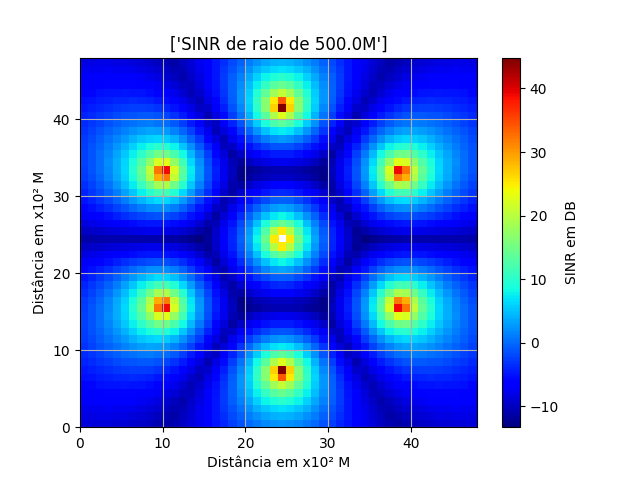
\includegraphics[width=0.75\textwidth]{REMSINR.png}
    \caption{}
    \label{fig:my_label}
\end{figure}
\FloatBarrier
Também foi pedido para mostrar o Gráfico das CDFs da SINR ,Taxa de transmissão e \textit{throughput} para o melhor caso do LTE, que é a banda de 20MHZ e mimo 4x4. Com isso conseguimos mostrar para os raios especificados de 50,100,500 e 1000 metros:
\begin{figure}[h!]
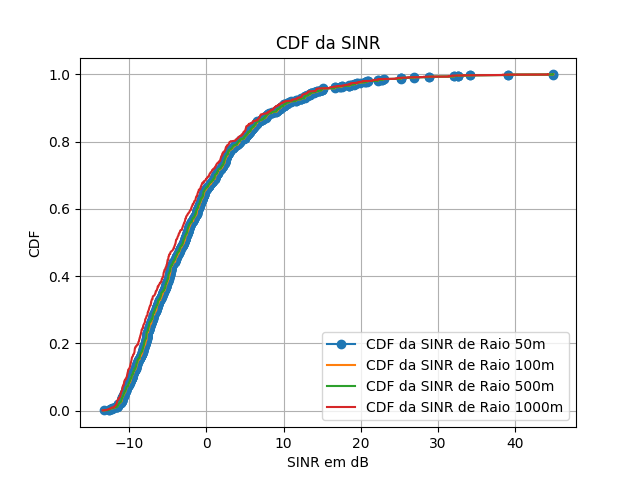
\includegraphics[width=0.95\textwidth]{CDF_SINR.png}
    \caption{CDF SINR}
    \label{fig:my_label}
\end{figure}
\FloatBarrier
\begin{figure}[h!]
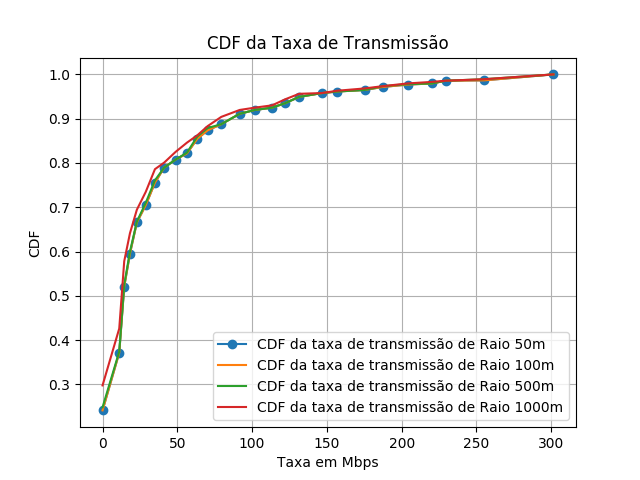
\includegraphics[width=0.95\textwidth]{CDF_Taxa_de_transmissao.png}
    \caption{CDF da taxa de transmissão}
    \label{fig:my_label}
\end{figure}
\FloatBarrier
\begin{figure}[h!]
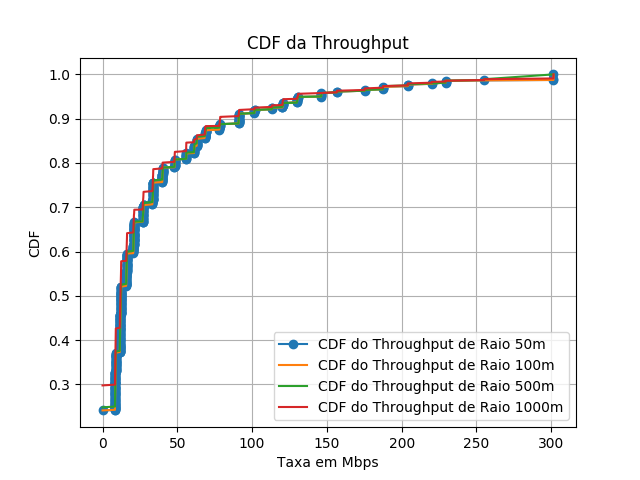
\includegraphics[width=0.95\textwidth]{CDF_Throughput.png}
    \caption{CDF do Throughput}
    \label{fig:my_label}
\end{figure}
\FloatBarrier
Os pontos em azul foram usados para diferenciar as CDFs de raio 50 e 100, porque estavam em cima do outro.lembrando que o Throughput é calculado com:
\begin{equation}
    Tput=TaxTrans*(1-BER)
\end{equation}
E a BER é calculada de acordo com a modulação que o MCS usa, e a SNR efetiva que é 90\% da SINR dada, e conseguimos calcular a BER pela formula para modulações M-QAM para quando $log_{2}(M)$ é par \cite{Lathi:2009:MDA:541365}:
\begin{equation}
    Pe=\frac{4}{log_{2}(M)}*(1-\frac{1}{\sqrt{M}})*Q\left ( \sqrt{\frac{3*log_{2}(M)*Eb/No}{M-1}} \right )


\end{equation}
Com os gráficos em mãos podemos perceber que quanto maior o Raio maior a quantidade de pontos com uma SNR, taxa de transmissão e  \textit{throughput} mais baixa. E na taxa de transmissão e throughput podemos ver que cerca de 20\% estão com 0Mbps isso é porque dada SNR 20\% estão fora da área de cobertura das ERBs. E quanto menor o Raio mais se concentram com MCS mais altas, fazendo assim uma maior taxa de transmissão.

Também foi pedido para que fosse mostrado as CDFs para os melhores e piores casos do Realease 8 e Release 10, foi escolhido o raio de 500m para mostrar e temos o seguinte:
\begin{figure}[h!]
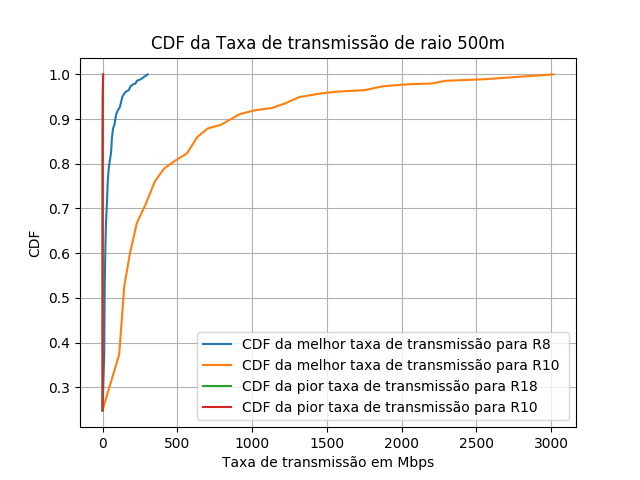
\includegraphics[width=0.95\textwidth]{CDF_especificos.png}
    \caption{CDF da Taxa de Transmissão para melhores e piores casos}
    \label{fig:my_label}
\end{figure}
\FloatBarrier
Como para os piores casos tem uma banda apenas de 1.4 Mhz,mimo 1x1 e prefixo cíclico estendido, e o melhor caso do release 10 tem 100Mhz de banda, mimo 8x8 e prefixo cíclico normal, é possível notar uma grande diferença a taxa de transmissão é cerca de mil vezes maior ou mais,por isso fica proximo do 0, e para o release 8 no melhor caso com 20Mhz de banda e mimo 4x4, podemos ver que chega apenas a 300Mbps, 10 vezes menos que a do release 10. Em comparação aos gráficos anteriores de gráficos o raio das ERBS não é um fator que faz tanta diferença em comparação com a quantidade de banda e mimo.

Também foi pedido para que fosse mostrado as CDFs do \textit{carrier aggregation} do release 10 e o melhor caso do release 8 com mimo 1x1 e prefixo cíclico normal. Com isso temos a imagem seguinte
\begin{figure}[h!]
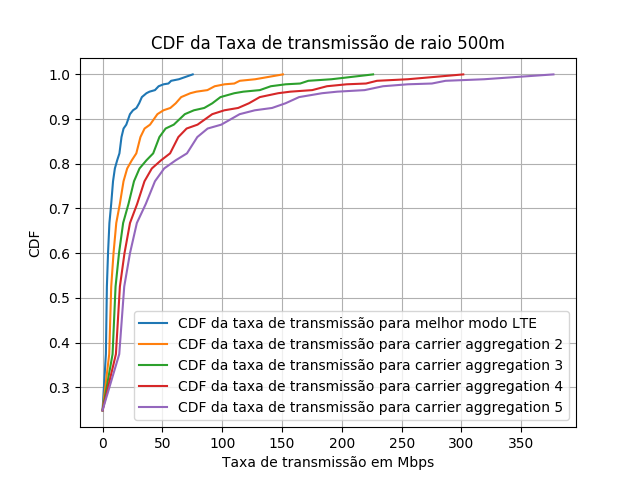
\includegraphics[width=0.95\textwidth]{CDF_Carrier.png}
    \caption{CDF da Taxa de Transmissão para Carrier aggregation}
    \label{fig:my_label}
\end{figure}
\FloatBarrier
Com essa imagem conseguimos perceber que quanto maior o carrier aggregation maior a taxa de transmissão, e quanto a comparação com vários raios, as condições dos parâmetros são os mesmos de calcular é a taxa de transmissão que na de varios raios elas terminam no mesmo ponto, já essa do carrier aggregation não.
\bibliographystyle{sbc}
\bibliography{sbc-template}
\end{document}
